% Fig. 1 -- AXIOM conceptual system view (vector, hand-drawn TikZ; no generative-AI content)
% Final size: 119 mm wide, the WPC maximum, at natural size. Helvetica 8--9 pt, no bold, no transparency (EPS stays vector).
% 2026-11-15: x unit 0.905 mm (was 1 mm) and box widths scaled to match, labels in the paper's own terms.
\documentclass[border=0.5mm]{standalone}
\usepackage[T1]{fontenc}
\usepackage[scaled=1]{helvet}
\renewcommand{\familydefault}{\sfdefault}
\usepackage[eulergreek]{sansmath}
\usepackage{tikz}
\usetikzlibrary{arrows.meta,calc,positioning,shapes.geometric,backgrounds,decorations.pathreplacing}
\definecolor{urllc}{HTML}{C4501B}
\definecolor{embb}{HTML}{1F5F9E}
\definecolor{mmtc}{HTML}{17785A}
\definecolor{clus}{HTML}{B85C00}
\definecolor{core}{HTML}{34418F}
\definecolor{ink}{HTML}{2B2B2B}
\definecolor{mute}{HTML}{8A8A8A}
\tikzset{
  >={Stealth[length=2.2mm,width=1.6mm]},
  every node/.style={font=\fontsize{8}{9.6}\selectfont\sansmath, text=ink},
  icon/.style={line width=0.55pt, draw=#1, line cap=round, line join=round},
  lbl/.style={font=\fontsize{8}{9.6}\selectfont\sansmath},
  ttl/.style={font=\fontsize{9}{10.8}\selectfont\sansmath},
  pics/gnb/.style={code={
    \begin{scope}[icon=#1]
      \draw (-1.7,0)--(0,9.2)--(1.7,0);
      \draw (-1.25,2.4)--(1.25,2.4) (-0.8,4.8)--(0.8,4.8) (-0.4,7.0)--(0.4,7.0);
      \draw (-1.25,2.4)--(0.8,4.8) (1.25,2.4)--(-0.8,4.8) (-0.8,4.8)--(0.4,7.0) (0.8,4.8)--(-0.4,7.0);
      \draw[fill=white] (-0.55,9.0) rectangle (0.55,10.6);
      \foreach \r in {1.7,2.7}{
        \draw (0,9.8) ++(40:\r) arc (40:-40:\r);
        \draw (0,9.8) ++(140:\r) arc (140:220:\r);}
    \end{scope}}},
  pics/server/.style={code={
    \foreach \y in {0,1.9,3.8}{
      \draw[icon=#1, fill=white, rounded corners=0.4mm] (0,\y) rectangle (6.2,\y+1.5);
      \fill[#1] (0.8,\y+0.75) circle (0.28) (1.7,\y+0.75) circle (0.28);
      \draw[icon=#1] (3.2,\y+0.75)--(5.4,\y+0.75);}}},
  pics/car/.style={code={
    \begin{scope}[icon=#1]
      \draw[fill=#1!12, rounded corners=0.8mm] (0,1)--(0,2.9)--(2.1,3.2)--(3.6,5.1)--(7.2,5.1)--(8.6,3.2)--(10.4,2.9)--(10.4,1)--cycle;
      \draw (3.9,3.3)--(4.3,4.6)--(5.3,4.6)--(5.3,3.3)--cycle (5.8,3.3)--(5.8,4.6)--(6.9,4.6)--(7.7,3.3)--cycle;
      \draw[fill=white] (2.5,1) circle (1.05) (7.9,1) circle (1.05);
      \fill[#1] (2.5,1) circle (0.35) (7.9,1) circle (0.35);
      \draw (5.4,6.0) ++(55:1.0) arc (55:125:1.0);
      \draw (5.4,6.0) ++(50:1.9) arc (50:130:1.9);
      \fill[#1] (5.4,6.0) circle (0.3);
    \end{scope}}},
  pics/drone/.style={code={
    \begin{scope}[icon=#1]
      \draw (-3.6,1.2)--(3.6,1.2);
      \draw (-3.6,1.2)--(-3.6,1.9) (3.6,1.2)--(3.6,1.9);
      \draw[fill=#1!12] (-3.6,2.15) ellipse (2.0 and 0.35) (3.6,2.15) ellipse (2.0 and 0.35);
      \draw[fill=#1!12, rounded corners=0.6mm] (-1.5,0.4) rectangle (1.5,2.0);
      \draw (-1.0,0.4)--(-1.6,-0.6)--(-2.2,-0.6) (1.0,0.4)--(1.6,-0.6)--(2.2,-0.6);
      \fill[#1] (0,1.2) circle (0.35);
    \end{scope}}},
  pics/robot/.style={code={
    \begin{scope}[icon=#1]
      \draw[fill=#1!12, rounded corners=0.4mm] (-2.2,0) rectangle (2.2,1.1);
      \draw[line width=1.6pt, draw=#1] (0,1.6)--(1.6,5.4)--(4.8,4.6);
      \draw[fill=white] (0,1.6) circle (0.7) (1.6,5.4) circle (0.65);
      \draw (4.8,4.6)--(5.3,5.4)--(6.2,5.5) (4.8,4.6)--(5.4,3.9)--(6.3,3.9);
    \end{scope}}},
  pics/phone/.style={code={
    \begin{scope}[icon=#1]
      \draw[fill=white, rounded corners=0.7mm] (0,0) rectangle (3.6,6.6);
      \draw[fill=#1!12] (0.4,0.9) rectangle (3.2,5.8);
      \fill[#1] (1.5,2.6)--(1.5,4.1)--(2.6,3.35)--cycle;
      \draw (1.3,0.45)--(2.3,0.45);
    \end{scope}}},
  pics/vr/.style={code={
    \begin{scope}[icon=#1]
      \draw (0.2,2.6) .. controls (1.5,4.9) and (7.5,4.9) .. (8.8,2.6);
      \draw[fill=#1!12, rounded corners=1.2mm] (0,0) rectangle (9,3.6);
      \draw[fill=white] (2.6,1.75) circle (1.1) (6.4,1.75) circle (1.1);
      \draw (4.0,0)--(4.5,0.9)--(5.0,0);
    \end{scope}}},
  pics/laptop/.style={code={
    \begin{scope}[icon=#1]
      \draw[fill=white, rounded corners=0.5mm] (1,1) rectangle (8.2,6.0);
      \draw[fill=#1!12] (1.5,1.5) rectangle (7.7,5.5);
      \draw[fill=white, rounded corners=0.3mm] (0,0)--(9.2,0)--(8.4,1)--(0.8,1)--cycle;
      \foreach \h [count=\i] in {1.0,1.8,1.3,2.4,2.0}{\fill[#1] (2.2+\i*0.9,1.9) rectangle ++(0.5,\h);}
    \end{scope}}},
  pics/meter/.style={code={
    \begin{scope}[icon=#1]
      \draw[fill=white, rounded corners=0.6mm] (0,0) rectangle (5.4,6.6);
      \draw[fill=#1!12] (2.7,4.1) circle (1.5);
      \draw (2.7,4.1)--++(50:1.2); \fill[#1] (2.7,4.1) circle (0.25);
      \draw[fill=#1!12] (0.8,0.8) rectangle (4.6,2.0);
      \foreach \x in {1.3,2.1,2.9,3.7}{\draw (\x,1.1)--(\x,1.7);}
    \end{scope}}},
  pics/sensor/.style={code={
    \begin{scope}[icon=#1]
      \draw[fill=#1!12, rounded corners=0.6mm] (-1.8,0) rectangle (1.8,3.0);
      \foreach \x in {-0.9,0,0.9}{\fill[#1] (\x,1.5) circle (0.3);}
      \draw (0,3.0)--(0,4.3); \fill[#1] (0,4.3) circle (0.3);
      \draw (0,4.3) ++(35:1.1) arc (35:-35:1.1) (0,4.3) ++(145:1.1) arc (145:215:1.1);
      \draw (0,4.3) ++(35:2.0) arc (35:-35:2.0) (0,4.3) ++(145:2.0) arc (145:215:2.0);
    \end{scope}}},
  pics/watch/.style={code={
    \begin{scope}[icon=#1]
      \draw[fill=#1!12] (0.9,-1.4) rectangle (3.1,7.4);
      \draw[fill=white, rounded corners=1mm] (0,1.2) rectangle (4,4.8);
      \draw (2,3.0)--(2,4.1) (2,3.0)--(2.9,2.6);
    \end{scope}}},
  pics/ue/.style={code={
    \draw[icon=#1, fill=white, rounded corners=0.6mm] (0,0) rectangle (3.0,5.4);
    \draw[icon=#1] (0.4,0.8) rectangle (2.6,4.7);}},
  pics/bolt/.style={code={\fill[#1] (0.9,3.2)--(0,1.4)--(0.8,1.4)--(0.3,0)--(1.6,2.0)--(0.8,2.0)--(1.3,3.2)--cycle;}},
  pics/bars/.style={code={\foreach \h [count=\i] in {1.0,1.8,2.6,3.2}{\fill[#1] (\i*0.75-0.75,0) rectangle ++(0.5,\h);}}},
  pics/dots/.style={code={\foreach \x in {0,0.9,1.8}{\foreach \y in {0,0.9,1.8}{\fill[#1] (\x,\y+0.5) circle (0.27);}}}},
}
\begin{document}
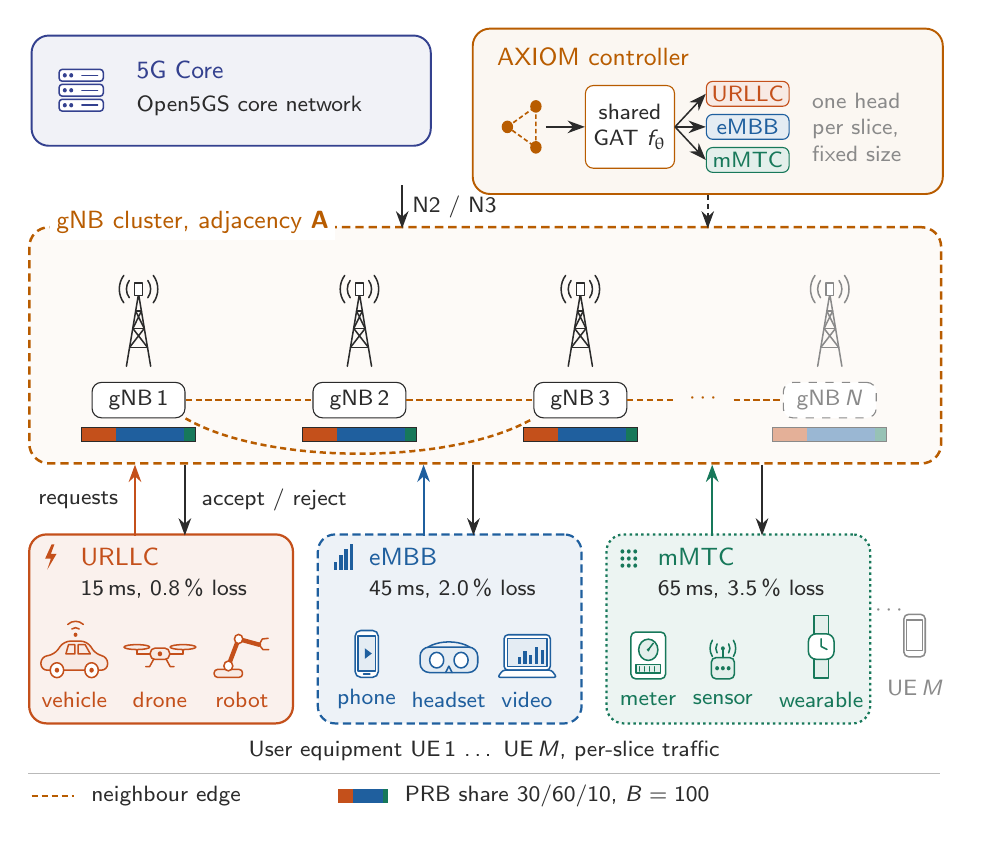
\begin{tikzpicture}[x=0.905mm,y=1mm]
\node[draw=core, line width=0.7pt, fill=core!7, rounded corners=2.2mm,
      minimum width=50.7mm, minimum height=14mm] (core) at (29,91.5) {};
\pic at ($(core.west)+(4,-2.6)$) {server=core};
\node[ttl, text=core, anchor=north west] at ($(core.north west)+(13.5,-2.2)$) {5G Core};
\node[lbl, anchor=north west] at ($(core.north west)+(13.5,-6.6)$) {Open5GS core network};
\node[draw=clus, line width=0.7pt, fill=clus!5, rounded corners=2.2mm,
      minimum width=59.7mm, minimum height=21mm, anchor=north east] (ctl) at (129,99.5) {};
\node[ttl, text=clus, anchor=north west] at ($(ctl.north west)+(2.2,-1.4)$) {AXIOM controller};
\coordinate (g0) at ($(ctl.north west)+(5,-12.6)$);
\begin{scope}[shift={(g0)}]
  \draw[clus, line width=0.6pt, dash pattern=on 1.6pt off 1pt] (0,0)--(4,2.6)--(4,-2.6)--cycle;
  \fill[clus] (0,0) circle (0.8) (4,2.6) circle (0.8) (4,-2.6) circle (0.8);
\end{scope}
\node[lbl, draw=clus, fill=white, rounded corners=1mm, align=center, inner sep=1mm,
      minimum height=10.5mm] (enc) at ($(g0)+(17.2,0)$) {shared\\GAT $f_\theta$};
\draw[->, ink, line width=0.6pt] ($(g0)+(5.4,0)$)--(enc.west);
\foreach \sl/\cl/\dy [count=\i] in {URLLC/urllc/4.2,eMBB/embb/0,mMTC/mmtc/-4.2}{
  \node[lbl, draw=\cl, fill=\cl!12, text=\cl, rounded corners=0.8mm, inner sep=0.6mm, minimum width=10.5mm]
       (qh\i) at ($(enc.east)+(10.2,\dy)$) {\sl};
  \draw[->, ink, line width=0.55pt] (enc.east)--(qh\i.west);}
\node[lbl, anchor=west, text=mute, align=left] at ($(qh2.east)+(1.8,0)$) {one head\\per slice,\\fixed size};
\node[draw=clus, line width=0.9pt, dash pattern=on 3pt off 1.8pt, rounded corners=2.5mm,
      minimum width=115.8mm, minimum height=30mm, anchor=south west, fill=clus!3] (clu) at (0.5,44) {};
\node[ttl, text=clus, anchor=south west, fill=white, inner sep=0.8mm] at ($(clu.north west)+(3,-1.8)$)
     {gNB cluster, adjacency $\mathbf{A}$};
\foreach \x/\name/\col/\tint/\bst [count=\i] in {16/gNB\,1/ink/100/solid, 47/gNB\,2/ink/100/solid, 78/gNB\,3/ink/100/solid, 113/gNB\,$N$/mute/45/dashed}{
  \pic at (\x,56.5) {gnb=\col};
  \node[lbl, draw=\col, text=\col, fill=white, rounded corners=1.2mm, minimum width=11.8mm, inner sep=1.0mm,
        \bst] (g\i) at (\x,52.2) {\name};
  \fill[urllc!\tint!white] (\x-8,47.0) rectangle ++(4.8,1.7);
  \fill[embb!\tint!white]  (\x-3.2,47.0) rectangle ++(9.6,1.7);
  \fill[mmtc!\tint!white]  (\x+6.4,47.0) rectangle ++(1.6,1.7);
  \draw[\col, line width=0.3pt] (\x-8,47.0) rectangle ++(16,1.7);
}
\begin{scope}[clus, line width=0.9pt, dash pattern=on 2.2pt off 1.4pt]
  \draw (g1.east)--(g2.west);
  \draw (g2.east)--(g3.west);
  \draw (g1.south east) .. controls (34,43.9) and (60,43.9) .. (g3.south west);
  \draw (g3.east)--(91,52.2);
  \draw (99.5,52.2)--(g4.west);
\end{scope}
\node[lbl, text=clus] at (95.2,52.4) {$\cdots$};
\draw[->, ink, line width=0.7pt] (53,79.5)--(53,74) node[midway, right, lbl] {N2 / N3};
\draw[ink, line width=0.6pt, dash pattern=on 2pt off 1.2pt, ->] (ctl.south)--(ctl.south |- 0,74);
\newcommand{\slicepanel}[6]{%
  \node[draw=#2, line width=0.8pt, #3, fill=#2!8, rounded corners=2.2mm,
        minimum width=33.5mm, minimum height=24mm, anchor=south west] (p#4) at (#1,11) {};
  \pic at ($(p#4.north west)+(2.4,-4.6)$) {#5=#2};
  \node[ttl, text=#2, anchor=west] at ($(p#4.north west)+(6.0,-3.0)$) {#4};
  \node[lbl, anchor=west] at ($(p#4.north west)+(6.0,-7.0)$) {#6};
}
\slicepanel{0.5}{urllc}{solid}{URLLC}{bolt}{15\,ms, 0.8\,\% loss}
\slicepanel{41}{embb}{dash pattern=on 3pt off 1.6pt}{eMBB}{bars}{45\,ms, 2.0\,\% loss}
\slicepanel{81.5}{mmtc}{dash pattern=on 0.9pt off 1.2pt}{mMTC}{dots}{65\,ms, 3.5\,\% loss}
\begin{scope}[every pic/.style={scale=0.9}]
\pic at (2.3,17.0) {car=urllc};
\pic at (19,18.9) {drone=urllc};
\pic at (28.6,17.0) {robot=urllc};
\pic at (46.4,17.0) {phone=embb};
\pic at (55.5,17.6) {vr=embb};
\pic at (66.4,17.0) {laptop=embb};
\pic at (85.1,16.8) {meter=mmtc};
\pic at (98,16.8) {sensor=mmtc};
\pic at (110,18.2) {watch=mmtc};
\end{scope}
\foreach \x/\t in {7/vehicle, 19/drone, 30.5/robot}{\node[lbl, text=urllc] at (\x,14.2) {\t};}
\foreach \x/\t in {48/phone, 59.5/headset, 70.5/video}{\node[lbl, text=embb] at (\x,14.2) {\t};}
\foreach \x/\t in {87.5/meter, 98/sensor, 111.8/wearable}{\node[lbl, text=mmtc] at (\x,14.2) {\t};}
\node[lbl, text=mute] at (121.3,25.5) {$\cdots$};
\pic at (123.4,19.6) {ue=mute};
\node[lbl, text=mute] at (125,15.6) {UE\,$M$};
\foreach \px/\cl in {19/urllc, 59.5/embb, 100/mmtc}{
  \draw[->, \cl, line width=0.7pt] (\px-3.5,35)--(\px-3.5,44);
  \draw[->, ink, line width=0.7pt] (\px+3.5,44)--(\px+3.5,35);}
\node[lbl, anchor=east] at (14.5,39.5) {requests};
\node[lbl, anchor=west] at (23.5,39.5) {accept / reject};
\node[lbl] at (64.5,7.6) {User equipment UE\,1 \ldots\ UE\,$M$, per-slice traffic};
\draw[mute!60, line width=0.3pt] (0.5,4.8)--(128.5,4.8);
\draw[clus, line width=0.9pt, dash pattern=on 2.2pt off 1.4pt] (1,1.9)--(7,1.9);
\node[lbl, anchor=west] at (8,1.9) {neighbour edge};
\fill[urllc] (44,1.05) rectangle ++(2.1,1.7);
\fill[embb]  (46.1,1.05) rectangle ++(4.2,1.7);
\fill[mmtc]  (50.3,1.05) rectangle ++(0.7,1.7);
\node[lbl, anchor=west] at (52,1.9) {PRB share 30/60/10, $B=100$};
\end{tikzpicture}
\end{document}
